% Created 2019-03-23 Sat 17:36
% Intended LaTeX compiler: pdflatex
\documentclass[a4paper, 12pt]{article}
\usepackage[utf8]{inputenc}
\usepackage[T1]{fontenc}
\usepackage{graphicx}
\usepackage{grffile}
\usepackage{longtable}
\usepackage{wrapfig}
\usepackage{rotating}
\usepackage[normalem]{ulem}
\usepackage{amsmath}
\usepackage{textcomp}
\usepackage{amssymb}
\usepackage{capt-of}
\usepackage{hyperref}
\usepackage[left=2.5cm, right=2.5cm, top=2.5cm, bottom=2.5cm, bindingoffset=1.5cm, head=15pt]{geometry}
\usepackage{setspace}
\usepackage{caption}
\onehalfspacing
\usepackage[official]{eurosym}
\usepackage{amsmath}
\usepackage{amssymb}
\usepackage{notation/rl}
\usepackage{notation/model}
\usepackage{template/informs}
\let\enumerate\henumerate
\let\itemize\hitemize
\usepackage{fancyhdr}
\pagestyle{fancy}
\fancyhead{}
\fancyfoot{}
\fancyhead[LE,RO]{\textsl{\leftmark}}
\fancyhead[RE,LO]{Tobias Richter}
\fancyfoot[C]{\thepage}
\renewcommand{\headrulewidth}{0.4pt}
\renewcommand{\footrulewidth}{0pt}
\usepackage{apacite}
\let\cite\shortcite
\let\textcite\shortciteA
\usepackage[nohyperlinks]{acronym}
\interfootnotelinepenalty=10000
\usepackage[notlof,notlot,nottoc]{tocbibind}
\newcommand{\studentID}{558305}
\newcommand{\thesistype}{Master Thesis}
\newcommand{\supervisor}{Univ.-Prof. Dr. Wolfgang Ketter}
\newcommand{\cosupervisor}{Karsten Schroer}
\pagenumbering{Roman}
\author{Tobias Richter}
\date{\today}
\title{Reinforcement Learning Portfolio Optimization of Electric Vehicle Virtual Power Plants}
\hypersetup{
 pdfauthor={Tobias Richter},
 pdftitle={Reinforcement Learning Portfolio Optimization of Electric Vehicle Virtual Power Plants},
 pdfkeywords={},
 pdfsubject={},
 pdfcreator={Emacs 26.1 (Org mode 9.2.1)},
 pdflang={English}}
\begin{document}

\makeatletter
\begin{titlepage}
    \begin{center}
        \vspace*{1cm}

        \Large
        \textbf{\@title{}}

        \vspace{1.5cm}

        \thesistype{}

        \vspace{1cm}

        \begin{figure}[htbp]
             \centering
             
\includegraphics[width=.5\linewidth]{./fig/UoC_Logo.png}
        \end{figure}

        \vspace{1cm}

        \large
        \textbf{Author}: \@author{} (Student ID: \studentID{})\\
        \large
        \textbf{Supervisor}: \supervisor{}\\
        \large
        \textbf{Co-Supervisor}: \cosupervisor{}

        \vspace{1cm}
        \large
        Department of Information Systems for Sustainable Society\\
        Faculty of Management, Economics and Social Sciences\\
        University of Cologne\\

        \vspace{1cm}
        \@date{}

    \end{center}
\end{titlepage}
\makeatother
\clearpage
\thispagestyle{empty}
\section*{Eidesstattliche Versicherung}
\label{sec:SOOA}

\vspace{2.5cm}

% Statement of original authorship - Needs to be in German
% see also here: https://www.wiso.uni-koeln.de/sites/fakultaet/dokumente/PA/formulare/eidesstattliche_erklaerung.pdf

Hiermit versichere ich an Eides statt, dass ich die vorliegende Arbeit selbstständig und ohne die Benutzung anderer als der angegebenen Hilfsmittel angefertigt habe. Alle Stellen, die wörtlich oder sinngemäß aus veröffentlichten und nicht veröffentlichten Schriften entnommen wurden, sind als solche kenntlich gemacht. Die Arbeit ist in gleicher oder ähnlicher Form oder auszugsweise im Rahmen einer anderen Prüfung noch nicht vorgelegt worden. Ich versichere, dass die eingereichte elektronische Fassung der eingereichten Druckfassung vollständig entspricht.

\vspace{1cm}

\noindent
Die Strafbarkeit einer falschen eidesstattlichen Versicherung ist mir bekannt, namentlich die Strafandrohung gemäß § 156 StGB bis zu drei Jahren Freiheitsstrafe oder Geldstrafe bei vorsätzlicher Begehung der Tat bzw. gemäß § 161 Abs. 1 StGB bis zu einem Jahr Freiheitsstrafe oder Geldstrafe bei fahrlässiger Begehung.

\vspace{3cm}
\noindent
\textbf{Tobias Richter}

\vspace{0.5cm}
\noindent
Köln, den 01.05.2019
\clearpage

\setcounter{page}{1}
\tableofcontents
\clearpage
\listoffigures
\clearpage
\listoftables
\clearpage

\section*{List of Abbreviations} \markboth{LIST OF ABBREVIATIONS}{}
\begin{acronym}[GCRM]
	\acro{ANN}{Artificial Neural Network}
	\acro{DP}{Dynamic Programming}
	\acro{DSO}{Distribution System Operator}
	\acro{EPEX}{European Power Exchange}
	\acro{EV}{Electric Vehicle}
	\acro{GCRM}{German Control Reserve Market}
	\acro{GP}{Genetic Programming}
	\acro{MAW}{Mean Asymmetric Weighted Objective Function}
	\acro{MC}{Monte Carlo}
	\acro{MDP}{Markov Decision Process}
	\acro{PDF}{Probability Density Function}
	\acro{RES}{Renewable Energy Sources}
	\acro{RL}{Reinforcement Learning}
	\acro{TD}{Temporal-Difference}
	\acro{TSO}{Transmission System Operator}
	\acro{V2G}{Vehicle-to-Grid}
	\acro{VPP}{Virtual Power Plant}
\end{acronym}
\clearpage
\section*{Summary of Notation} \markboth{SUMMARY OF NOTATION}{}
Capital letters are used for random variables, whereas lower case letters are used for
the values of random variables and for scalar functions. Quantities that are required to
be real-valued vectors are written in bold and in lower case (even if random variables).
\begin{tabbing}
    \=~~~~~~~~~~~~~~~~~~  \= \kill
    \>$\defeq$            \> equality relationship that is true by definition\\
    \>$\approx$           \> approximately equal\\
    \>$\E{X}$             \> expectation of a random variable $X$, i.e., $\E{X}\defeq\sum_x p(x)x$\\
    \>$\Re$               \> set of real numbers\\
    \>$\leftarrow$        \> assignment\\
    \\
    \>$\e$                \> probability of taking a random action in an \e-greedy policy\\
    \>$\alpha$            \> step-size parameter\\
    \>$\gamma$            \> discount-rate parameter\\
    \>$\lambda$           \> decay-rate parameter for eligibility traces\\
    \\
    \>$s, s'$             \> states\\
    \>$a$                 \> an action\\
    \>$r$                 \> a reward\\
    \>$\S$                \> set of all nonterminal states\\
    \>$\A$                \> set of all available actions\\
    \>$\R$                \> set of all possible rewards, a finite subset of $\Re$\\
    \>$\subset$           \> subset of; e.g., $\R\subset\Re$\\
    \>$\in$               \> is an element of; e.g., $s\in\S$, $r\in\R$\\
    \\
    \>$t$                 \> discrete time step\\
    \>$T, T(t)$           \> final time step of an episode, or of the episode including time step $t$\\
    \>$A_t$               \> action at time $t$\\
    \>$S_t$               \> state at time $t$, typically due, stochastically, to $S_{t-1}$ and $A_{t-1}$\\
    \>$R_t$               \> reward at time $t$, typically due, stochastically, to $S_{t-1}$ and $A_{t-1}$\\
    \>$\pi$               \> policy (decision-making rule)\\
    \>$\pi(s)$            \> action taken in state $s$ under {\it deterministic\/} policy $\pi$\\
    \>$\pi(a|s)$          \> probability of taking action $a$ in state $s$ under {\it stochastic\/} policy $\pi$\\
    \>$G_t$               \> return following time $t$\\
    \\
    \>$\p(s',r|s,a)$      \> probability of transition to state $s'$ with reward $r$, from state $s$ and action $a$\\
    \>$\p(s'|s,a)$        \> probability of transition to state $s'$, from state $s$ taking action $a$\\
    \>$\vpi(s)$           \> value of state $s$ under policy $\pi$ (expected return)\\
    \>$\vstar(s)$         \> value of state $s$ under the optimal policy\\
    \>$\qpi(s,a)$         \> value of taking action $a$ in state $s$ under policy $\pi$\\
    \>$\qstar(s,a)$       \> value of taking action $a$ in state $s$ under the optimal policy\\
    \>$V, V_t$            \> array estimates of state-value function $\vpi$ or $\vstar$\\
    \>$Q, Q_t$            \> array estimates of action-value function $\qpi$ or $\qstar$\\
    \\
    \>$d$                 \> dimensionality---the number of components of $\w$\\
    \>$\w$                \> $d$-vector of weights underlying an approximate value function\\
    \>$\hat v(s,\w)$      \> approximate value of state $s$ given weight vector $\w$\\
    \>$\mu(s)$            \> on-policy distribution over states\\
    \>$\MSVEm$            \> mean square value error\\
\end{tabbing}
\clearpage

\pagenumbering{arabic}

\section{Model: FleetRL}
\label{sec:org03b19ea}
The following chapter will introduce the model of this research. In its essence,
we propose a solution for EV fleet providers to utilize a VPP portfolio to
profitably provide balancing services to the grid on multiple markets. A control
mechanism procures energy from electricity markets, allocates available EVs to
VPPs, and intelligently dispatches EVs to charge the acquired amount of energy.
The model uses a RL agent that learns an optimal bidding strategy by interacting
with the electricity markets and reacts to changing rental demand of the EV
fleet. This chapter is structured as follows: The information assumptions are
listed first, the control mechanism is explained next, and finally the RL
approach is described in detail. For a table of notation refer to Table
\ref{table-notation}.

We formulate the problem as a \emph{controlled EV charging} problem. The EV fleet
operator represents the \emph{controller}, which aims to charge the fleet at minimal
costs. First, the controller predicts the amount of energy it can charge in a
given \emph{market period} \(h\). The length of the market period \(\Delta h\) and the
market closing time depend on the considered electricity market. Second, the
controller places bids on one or multiple markets to procure the predicted
amount of energy. Lastly, at electricity delivery time, the controller
communicates with the EV fleet to control the charging in real-time. Online EV
\emph{control periods} \(t\) are typically shorter than market periods. In the
empirical case that we consider, the market periods are 15 minutes long, while
the EV control periods last 5 minutes. Nonetheless, the presented approach
generalizes to other period lengths. During each control period, the controller
has to take decisions which individual EVs it should dispatch to charge the
procured amount of electricity. In times of unforeseen rental demand, this
decision implies trading off commitments to the markets with compromising
customer mobility by refusing customer rentals.


\begin{longtable}{l|p{0.7\linewidth}|l}
\caption[Table of Notation]{Table of Notation \label{table-notation}}
\\
\hline
\hline
Symbol & Description & Unit\\
\hline
\endfirsthead
\multicolumn{3}{l}{Continued from previous page} \\
\hline

Symbol & Description & Unit \\

\hline
\endhead
\hline\multicolumn{3}{r}{Continued on next page} \\
\endfoot
\endlastfoot
\hline
\(t\) & Control period. & -\\
\(h\) & Market period. & -\\
\(T\) & Number of control periods in a market period. & -\\
\(H\) & Number of market periods in day. & -\\
\(N_h\) & Total number of market periods. & -\\
\(\Delta t\) & Length of control period. & hours\\
\(\Delta h\) & Length of market period. & hours\\
\hline
\(\Pb{h}\) & Amount of balancing power offered on the balancing market. & kW\\
\(\cp{h}\) & Capacity price offered on the balancing market. & \(\emw\)\\
\(\ep{h}\) & Energy price offered on the balancing market. & \(\emwh\)\\
\(\ccp{h}\) & Critical capacity price in market period \(h\). & \(\emw\)\\
\(\cep{h}\) & Critical energy price in market period \(h\). & \(\emwh\)\\
\hline
\(\Pi{h}\) & Amount of power offered for the unit on the intraday market. & kW\\
\(\up{h}\) & Unit price offered on the intraday market. & \(\emwh\)\\
\(\cup{h}\) & Critical unit price in market period \(h\). & \(\emwh\)\\
\hline
\(\Eb{h}\) & Amount of energy charged from balancing market in market period h. & MWh\\
\(\Ei{h}\) & Amount of energy charged from the intraday market in market period h. & MWh\\
\(p^{i}\) & Industry tariff & \(\ekwh\)\\
\hline
\(\fP{t}\) & Amount of available fleet charging power in control period \(t\). & kW\\
\(\fPhat{t}\) & Predicted amount of available fleet charging power in control period \(t\). & kW\\
\hline
\(\Cb{h}(P)\) & Cost function for procuring electricity from the balancing market. & \(\eur\)\\
\(\Ci{h}(P)\) & Cost function for procuring electricity from the intraday market. & \(\eur\)\\
\(\oc\) & Opportunity costs of lost rental of EV \(i\) in control period \(t\). & \(\eur\)\\
\(\beta_h\) & Imbalance costs in market period \(h\). & \(\eur\)\\
\hline
\(\lb{h}\) & Balancing market risk factor. & -\\
\(\li{h}\) & Intraday market risk factor. & -\\
\(\theta_{\lambda}\) & Set of risk factors for all market periods \(h\!\in\!\{1,...,N_h\}\). & -\\
\(\Cf{}(\theta_{\lambda})\) & Cost function for the fleets total costs over all market periods \(h\). & \(\eur\)\\
\(\Cf{h}\) & Total accumulated fleet costs at market period \(h\). & \(\eur\)\\
\hline
\(i\) & Electric Vehicle. & -\\
\(\c\) & Dummy variable if EV is connected to a charging station. & 0/1\\
\(\omega_{i}\) & Amount of electricity stored in EV. & \(\kwh\)\\
\(\Omega\) & Maximum battery capacity of EV. & \(\kwh\)\\
\(\delta\) & Charging power of EV at the charging station. & \(\kw\)\\
\(\F\) & Set of all EVs in the fleet & -\\
\(\nF\) & Total number of EVs in the fleet. & -\\
\hline
\end{longtable}

\subsection{Required Information Assumptions \label{sec-model-assumptions}}
\label{sec:org0aefb0a}
The following information is assumed to be available:

\begin{enumerate}
\item The controller is able to forecast the mobility demand of the EV fleet at
different time-horizons based on historical data. More specifically, it can
predict the amount of plugged-in EVs and consequently the available charging
power \(P^{fleet}_t\) of the fleet at control period \(t\). The prediction's
accuracy is increasing with shorter time horizons, from uncertain predictions
one week ahead to very accurate predictions 30 minutes ahead. Past research
presented successful mobility demand forecast algorithms in the context of
free-float carsharing
\cite{kahlen18_elect_vehic_virtual_power_plant_dilem,kahlen17_fleet,wagner16_in_free_float}.
\item The controller is able to forecast electricity prices of spot and balancing
markets based on historical data. More specifically, it can estimate the
critical prices \(\ccp{h}\), \(\cep{h}\), and \(\cup{h}\) for each market period
with perfect accuracy. The critical prices form an essential piece of
information for the proposed bidding strategy; bids equal or below the
critical price will get accepted and result in successful electricity
procurement. Electricity price forecasting is an extensively studied
research area, with well-advanced prediction algorithms
\cite{weron14_elect_price_forec,avci18_manag_elect_price_model_risk}.
\end{enumerate}
We are confident that taking the above assumptions is viable, assuming available
forecasting information is common practice in the VPP and EV fleet charging
literature, see e.g.:
\textcite{brandt17_evaluat_busin_model_vehic_grid_integ,vandael15_reinf_learn_heuris_ev_fleet,mashhour11_biddin_strat_virtual_power_plant_1,tomic07_using_fleet_elect_drive_vehic_grid_suppor,pandzic13_offer_model_virtual_power_plant}.

\subsection{Control Mechanism}
\label{sec:org7a2a79f}
The central control mechanism constitutes the core of this research. It can be
seen as a decision support system that can be deployed at a EV fleet operator to
control the charging its fleet. Figure \ref{fig-control-mechanism} depicts the
control mechanism, which is divided into three distinct phases:

The first phase, \emph{Bidding Phase I}, takes place just before the closing time of
the balancing market, once every week (e.g., Wednesdays at 3pm at the GCRM). In
this phase, the controller can place bids for every market period \(h\) of the
following week on the balancing market. The second phase, \emph{Bidding Phase II},
takes places in every market period of \(\Delta{h}\!=\!15\) minutes. At this
point, the controller has the opportunity to place bids for the market period 30
minutes ahead. By submitting bids 30 minutes ahead of time, the controller
assures that the bid will be matched until the lead time of the market (e.g, 5
minutes on the EPEX Spot Intraday Continuous). The third phase, \emph{Dispatch
Phase}, takes places in every control period of \(\Delta{t}\!=\!5\) minutes. In
this phase the controller has to dispatch available EVs to charge the procured
electricity from the markets. This phase involves allocating individual EVs to
the VPP and eventually refusing customer rentals to assure that all commitments
can be fulfilled.

The following chapters will highlight the important parts of the various phases
and provide detailed explanation and mathematical formulations.

\begin{figure}[p]
\centering
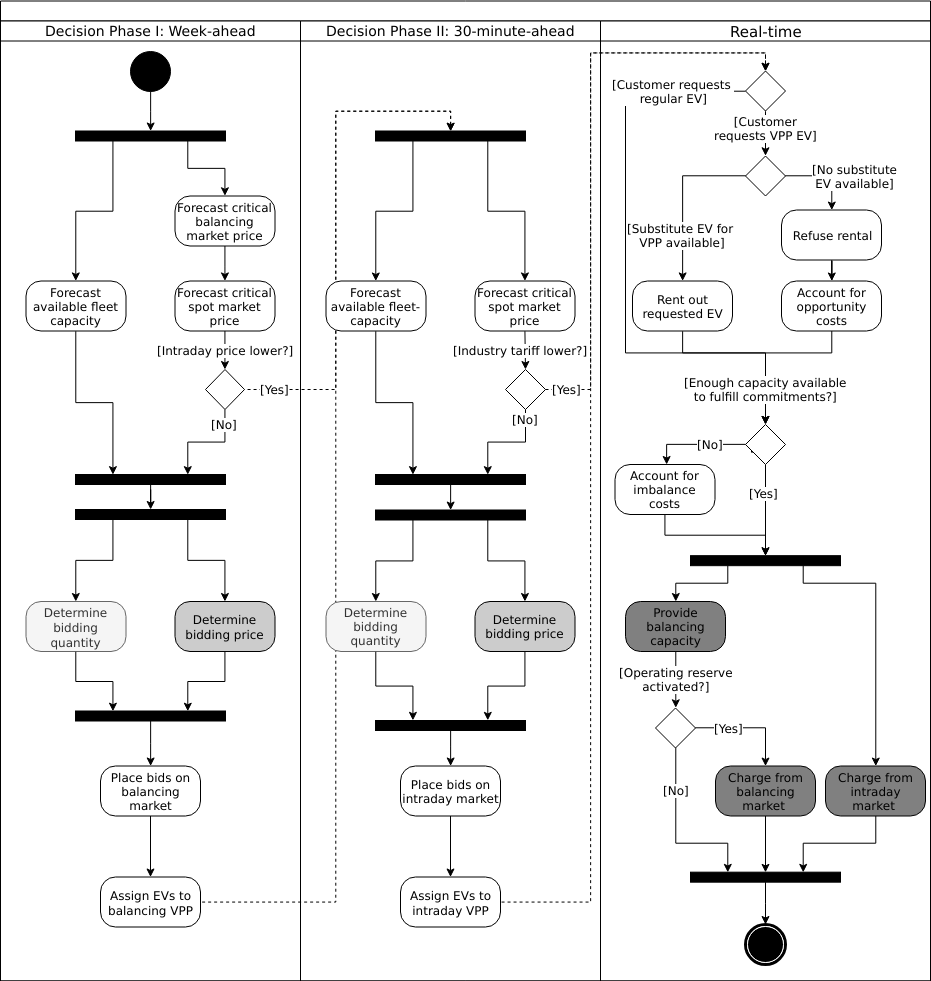
\includegraphics[width=1\linewidth]{./fig/control_mechanism.png}
\caption[EV VPP Control Mechanism]{EV VPP Control Mechanism \label{fig-control-mechanism}}
\end{figure}

\subsubsection{Fleet Charging Power Prediction}
\label{sec:org18d8b6a}
In a first step, the controller has to predict the available fleet charging
power \(\fPhat{h}\) for all market periods \(h\) of the next week. The actual
available fleet charging power \(\fP{t}\) in a control period \(t\) is given by the
number of EVs that are connected to a charging station, with enough free battery
capacity to charge the next control period \(t\!+\!1\). As mentioned in the
Chapter \ref{sec-model-assumptions}, the controller is able to predict the
available fleet charging power \(\fPhat{t}\) for all control periods \(t\) with
different levels of accuracy dependent on the time horizon of \(t\).

When the controller procures electricity from the markets, the fleet has to
charge with the committed charging power during all \(T\) control periods of the
market period \(h\).
To minimize the risk of not being able to charge the committed amount of energy
during the whole market period, and consequently causing imbalance costs, the
predicted fleet charging power in a market period is defined as the minimal
predicted fleet charging power of all \(T\) control periods in a market period.
\begin{equation}
    \fPhat{h} \defeq \min_{n \in \{1, .., T\}} \fPhat{t + n} \text{ ,}
\end{equation}
where \(h\) is the market period of interest and \(t\) its first control period.

\subsubsection{Market Decision}
\label{sec:orge75392b}
In a second step, the controller has to decide from which market it should
procure the desired amount of energy. Therefore, it compares the costs for
charging electricity from the balancing market and the intraday market. The cost
function for charging electricity from the balancing market is defined as follows:
\begin{equation} \label{eq-cost-balancing}
\begin{split}
    \Cb{h}(P) &\defeq -(P\!\times\!10^{-3} \times \ccp{h}) + (\Eb{h} \times \cep{h}) \\
    &= -(P\!\times\!10^{-3} \times \ccp{h}) + (P \frac{\Delta h}{10^{3}} \times \cep{h}) \text{ ,}
\end{split}
\end{equation}
where \(P\) (kW) is the amount of offered balancing power. The first term of the
equation corresponds to the compensation the controller retrieves for keeping
the balancing capacity available, while the second term corresponds to the costs
for charging the activated balancing energy \(\Eb{h}\) (MWh). Energy is power over
time, hence \(\Eb{h}\) can be substituted with \(P\) times the market periods length
\(\Delta{h}\), divided by the unit conversion from kW to MW. As mentioned in the
Chapter \ref{sec-model-assumptions}, the critical prices \(\ccp{}, \cep{}, \cup{}\)
are assumed to be available for all market periods. Note that the critical
energy price \(\cep{}\!\in\!\Re\), can also take negative values, resulting in
profits for the fleet, while the critical capacity price \(\ccp{}\!\in\! \Re^+_0\)
can not take negative values and therefore always results in profits for the
fleet.

The cost function for charging from the intraday market is defined similarly:
\begin{equation}
\begin{split}
    \Ci{h}(P) &\defeq \Ei{h} \times \cup{h} \\
    &= P \frac{\Delta h}{10^{3}}\times \cup{h}
\end{split}
\end{equation}
Again, depending on the market situation, \(\cup{}\!\in\!\Re\) can be either
negative or positive, resulting in costs or profits for the fleet. Contrarily to
the balancing market, on the intraday market the fleet does not get compensated
for keeping the charging power available; only the charged energy affects the
costs. If the costs for charging from the balancing market 7 days ahead
\(\Cb{h+(7\!\times\!H)}(\fPhat{h+(7\!\times\!H)})\) are higher than the costs of
charging from the intraday market at the same market period \(\Ci{h +
(7\!\times\!H)}(\fPhat{h+(7\!\times\!H)})\), the controller does not place bids
on the balancing market.

\subsubsection{Determining the Bidding Quantity}
\label{sec:org6feea74}
In a third step, the controller has to take a decision on the amount of energy
it should procure from the markets. Determining the bidding quantity is a
central piece of the controlled charging problem. The bidding quantity
determines the profits that can be made, by charging at a cheaper market price
than the flat industry tariff. In order to maximize its profits, the controller
aims to procure as much electricity as possible from the markets. In order to
optimally place bids on the electricity markets, it needs to balance the risk of
(a) procuring more energy that it can maximally charge and (b) not procuring
enough energy from the market to sufficiently charge the fleet.

In the first case (a), the fleet is facing costs of compromising customer
mobility, or worse, high imbalance penalties from the markets. Renting out EVs
is considerably more profitable than using EVs as a VPP to participate on the
electricity markets. Refusing customer rentals, in order to fulfill market
commitments, induces opportunity costs of lost rentals \(\rho\) on the fleet.
Imbalance costs \(\beta\) occur, when the fleet can not charge the committed
amount energy at all, even with refusing rentals. In the second case (b), the
fleet also faces opportunity costs of lost rentals when individual EVs do now
have enough SoC for planned trips of arriving customers.

The controller faces additional risks by bidding one week ahead on the balancing
market, in contrast to only 30 minutes ahead on the intraday market, as the
predictions of available charging power are more uncertain with the larger time
horizon. To account for all the mentioned risks, we introduce a \emph{risk factor}
\(\lambda \in \Re_{0 \leq \lambda \leq 1}\), where \(\lambda = 0\) indicates no
risk, and \(\lambda = 1\) indicates a high risk. The controller determines the
bidding quantity \(\Pb{h}\) by discounting the predicted available fleet charging
power \(\fPhat{h}\) with the possible risk \(\lambda_{h}\) of imbalance or
opportunity costs:
\begin{equation} \label{eq-model-pb}
  \Pb{h} \defeq
  \begin{cases}
    0, & \text{if}\ \Cb{h}(\fPhat{h}) \geq \Eb{h}10^3 \times p^{i}\\
    0, & \text{if}\ \Cb{h}(\fPhat{h}) \geq \Ci{h}(\fPhat{h})\\
    \fPhat{h} \times (1\!-\!\lb{h}), & \text{otherwise}
  \end{cases}
\end{equation}
where \(h\) is the market period of interest one week ahead. If the controller can
buy electricity at the intraday market at a lower price, it does not place a bid
at the balancing market. If the controller can charge cheaper at the regular
industry tariff \(p^{i}\), it does not place a bid either. In all other cases, the
controller submits \(\Pb{h}\) to the market.

The bidding quantity for the intraday market \(\Pi{h}\) depends on the previously
committed charging power \(\Pb{h}\) and the newly predicted charging power
\(\fPhat{h}\):
\begin{equation} \label{eq-model-pi}
  \Pi{h} \defeq
  \begin{cases}
    0, & \text{if}\ \Ci{h}(\fPhat{h}\!-\!\Pb{h}) \geq \Ei{h}10^3 \times p^{i}\\
    (\fPhat{h}\!-\!\Pb{h}) \times (1\!-\!\li{h}), & \text{otherwise}
  \end{cases}
\end{equation}
where \(h\) is the market period of interest 30 minutes ahead. Note that any
amount of electricity that the controller procured from the balancing market,
does not need to be bought from intraday market for the same market period.
Since the predicted charging power \(\fPhat{h}\) is expected to be more
accurate 30 minutes ahead than one week ahead, the controller is able to correct
bidding errors it made in the first decision phase, and optimally charge the
whole EV fleet.

\subsubsection{Dispatching Electronic Vehicle Charging}
\label{sec:org84fc420}
In the last step, at electricity delivery time, the EVs have to be assigned to
the VPP and be \emph{dispatched} to charge. Therefore the controller first needs to
detect how many EVs are eligible to be used as VPP per control period \(t\). EVs
are eligible if they (a) are connected to a charging station (\(\c\)), and (b)
have enough free battery storage available (\(\Omega\!-\!\omega_{i}\)) to charge
the next control period. Hence, the VPP is defined as:
\begin{equation}
    VPP \defeq \{i\;|\;i\in\F \vee \c = 1 \vee \Omega\!-\!\omega_{i}\!\geq\!\gamma\Delta{t}\} \text{ ,}
\end{equation}
where \(\gamma\Delta{t}\) (kWh) denotes the amount of energy that can be charged
with the charging speed of \(\gamma\) (kW) in control period \(t\).

Remember that the fleet has to provide the committed charging power
\(\Pb{h}\!+\!\Pi{h}\) across all control periods \(t\) of the market period \(h\),
independent of which individual EVs are actually charging the electricity. This
fact allows the controller to dynamically dispatch EVs every control period and
react to unforeseen rental demand. If a customer want to rent out an EV that is
assigned to the VPP, the controller only has to refuse the rental, if no other
EV is available to charge instead. When no replacement EV is available, the
controller has to account for lost rental profits \(\oc\). If the VPPs total
amount of available charging power \(|VPP|\!\times\!\gamma\) is not sufficient to
provide the total market commitments \(\Pb{h}\!+\!\Pi{h}\), the fleet gets charged
imbalance costs \(\beta_{h}\). Otherwise all the committed energy can be charged
by the VPP.

\subsubsection{Evaluating the Bidding Risk}
\label{sec:orgc0b3bd2}
The controllers central goal is to choose the risk factors \(\lb{h}\), \(\li{h}\)
for every market period \(h\), that minimize the cost of charging, while avoiding
the risks of lost rental profits \(\oc\) or imbalance costs \(\beta_h\). The total
fleet costs are defined as follows:
\begin{equation} \label{eq-model-fleetcosts}
    \Cf{}(\theta_{\lambda}) \defeq \sum^{N_h}_h
    \bigg[ \Cb{h}(\Pb{h}) + \Ci{h}(\Pi{h}) + \beta_{h}
    + \sum_t^{T} \sum_i^{\nF} \oc \bigg] \text{ ,}
\end{equation}
where \(\theta_{\lambda}\!\in\!\Re_{0 \leq \lambda \leq 1}^{2 \times N_h}\) is the
matrix of the risk factors \(\lb{h}\), \(\li{h}\) for all considered market periods
\(N_h\). \(\F\) denotes the set of all EVs \(i\) in the fleet and \(\nF\) the fleet
size. The costs for charging \(\Cb{h}(\Pb{h})\), \(\Ci{h}(\Pi{h})\) are clearly
dependent on the chosen risk factors \(\lb{h}\), \(\li{h}\) (see Eq.
\ref{eq-model-pb}, Eq. \ref{eq-model-pi}). In summary, the problem can be formulated
as minimizing the total costs of the fleet, by choosing the optimal set of risk
factors \(\theta_{\lambda}\):
\begin{equation}
\begin{aligned}
    & \underset{\theta_{\lambda}}{\text{minimize}}
    && \Cf{}(\theta_{\lambda}) \\
    & \text{subject to}
    && 0 \leq \lb{h} \leq 1, \; \forall \lb{h} \in \theta_{\lambda}\\
    &&& 0 \leq \li{h} \leq 1, \; \forall \li{h} \in \theta_{\lambda}\\
\end{aligned}
\end{equation}
Solving this optimization problem with common methods like stochastic
programming is a difficult task, assuming that complete information of available
charging power and future electricity market prices is not always available.
Since one goal of this research is to develop a model that can be applied to
previously unknown settings and learn from uncertain environments, as mobility
and electricity markets, we chose to solve the problem with a RL learning
approach that is explained in detail in Chapter \ref{sec-model-rf}.

\subsubsection{Example}
\label{sec:orgff0a933}
At 3pm on the 9\textsuperscript{th} of August 2017, the controller enters the first bidding
phase for procuring electricity one week ahead, the market period \(h\) =
\emph{16.08.2017 15:00-15:15}. It predicts that at that point in time 250 EVs are connected
to a charging station, resulting in 900kW available fleet charging power
(\(\fPhat{h}\!=\!900\kw\)), given the charging power of 3.6kW per EV. Assuming the
available critical prices \(\ccp{h}\!=\!5\emw\), \(\cep{h}\!=\!-10\emwh\), and
\(\cup{h}\!=\!10\emwh\) for that market period, the controller now evaluates the
cheapest charging option. The flat industry electricity tariff is assumed to be
\(p_i\!=\!0.15\ekwh\). The costs for charging with the maximal amount of power
\(\fPhat{h}\) from the balancing market (\(\Cb{h}(900\kw)\!=\!-6.25\eur\)) are less
than charging from the intraday market (\(\Ci{h}(900\kw)\!=\!2.25\eur\)) or
charging at the industry tariff
(\(900\kw\!\times\!0.25\text{h}\!\times\!0.15\ekwh\!=\!33.75\eur\)). In this
example, by choosing the cheapest option, the balancing market, the fleet
operator will even get compensated for charging its fleet.

In the next step, the controller has to submit bids to the balancing market. The
RL agent determined that the risk of bidding on the balancing market is
\(\lb{h}\!=\!0.3\). Consequently, the controller sets the bidding quantity to
\(\Pb{h}\!=\!\fPhat{h}\!\times\!(1\!-\!\lb{h})\!=\!900\kw\!\times0.7\!=\!630\kw\) and
submits a bid to the market. Since we are assuming that bids at the critical
price, will always get accepted, the controller procures 630kW from the
balancing market and updates its account with \(\Cb{h}(630\kw)\!=\!-4.725\eur\).

One week later, at 2:30pm on the 16\textsuperscript{th} of August 2017, the controller enters
the second bidding phase. With a time horizon of 30 minutes, it predicts less
available fleet charging power of \(\fPhat{h}\!=\!810\kw\) for the same market
period \emph{16.08.2017-15:00}. By trading at the intraday market, the controller can
now charge the remaining available EVs with a low risk of procuring more energy
than it can maximally charge. At this point in time, the RL agent determines a
remaining risk of \(\li{h}\!=\!0.05\), and sets the bidding quantity to
\(\Pi{h}\!=\!(810\kw\!-\!630\kw)\!\times\!(1\!-\!0.05)\!=\!171\kw\). Hence, the
controller procures 171kW from the intraday market and updates its account with
\(\Ci{h}(171\kw)\!=\!0.4275\eur\).

At electricity delivery time, the 16\textsuperscript{th} of August 2017 at 3:00pm, the
controller detects 255 available EVs; EVs which are connected to a charging
station and have enough battery capacity left to be charged in the next control
period. It assigns 223 EVs to provide the committed 801kW charging power for the
market period time \(\Delta h\) of 15 minutes. During that time, three customers
want to rent out EVs that are allocated to the VPP. The first two rentals are
accepted, because two other EVs are available to charge instead. The third
rental has be to refused, since no EV is remaining as substitution. The
controller has to account for the opportunity costs of the lost rental
\(\oc\).
\subsection{Reinforcement Learning Approach \label{sec-model-rf}}
\label{sec:orgd7fbd73}
In the following chapter the developed RL approach is outlined. First, the we
define the previously explained charging problem as a MDP, second, the used
learning algorithm is explained, and third, we give implementation and training
details.

Remember that the goal of the controlled charging problem is to choose a set of
risk factors \(\theta_{\lambda}\) that minimize the fleets total costs across all
market periods. The controllers can influencing the charging costs, by setting
the risk factors \(\li{}\), \(\lb{}\), which determine the bidding quantities \(\Pb{}\),
\(\Pi{}\). The controller has the possibility to submit bids to the markets every
market period \(h\). Hence, the RL agent has to take an action (i.e., determining
the risk factors) every timestep of \(t = h\).

The agent does so, by learning a policy \(\pi(a|s)\) that maps every state
\(s\in\S\) to an action \(a\in\A\). After the training period, the agent takes
action \(a\) whenever it observes a state \(S_t \in \S\).

\subsubsection{Markov Decision Process Definition}
\label{sec:org5edb05d}


\begin{itemize}
\item \(a \in A\)

\item Both bidding risk dependent on how many EVs available at that point in time
\item Both bidding risk dependent on daytime in hours at that point in time
\item Intraday Bidding risk dependent on how many EVs are available now
\end{itemize}


\begin{equation}
    \vpphat{t} \defeq \left\lceil\frac{\fPhat{t}}{\gamma}\right\rceil
\end{equation}

The state space is modeled with the dimensions 1) Predicted charging power
week-ahead, 2) time of the day of market period \(h\). The risk of bidding on the
markets is expected to be

\begin{equation}
    \S \defeq \left\{h(t), |VPP|_t, \vpphat{t+2}, \vpphat{t+(7\!\times\!H)}\right\}
\end{equation}
where:
\begin{itemize}
\item \(h(t)\) is the current daytime in hours, with discrete values in the range
\(\big[0,\;23\big] \in \Ne\).
\item \(|VPP|_t\) is the current VPP size, with discrete values in the range
\(\big[0,\;|\F|\big] \in \Ne\).
\item \(\vpphat{t+2}\) is the predicted VPP size 30 minutes ahead, with discrete values in the range
\(\big[0,\;|\F|\big] \in \Ne\).
\item \(\vpphat{t+(7\!\times\!H)}\) is the predicted VPP size 7 days ahead, with discrete
values in the range \(\big[0,\;|\F|\big] \in \Ne\).
\end{itemize}

Results in \(|\F|^3\!\times\!24 = 3\!\times\!10^9\) states.


\begin{itemize}
\item See \cite{reddy11_strat} for State/Action notation
\end{itemize}

Controller takes an action every
\begin{equation}
    \A \defeq \{\lb{t}, \li{t}\}
\end{equation}
where:
\begin{itemize}
\item \(\lb{t}\) is the risk factor for bidding on the balancing market, with discrete
values in the range \(\big[0,1\big]\) in 0.1 increments.
\item \(\li{t}\) is the risk factor for bidding on the intraday market, with discrete
values in the range \(\big[0,1\big]\) in 0.1 increments.
\end{itemize}

Results in \(10^2 = 100\) actions.


We define the reward function as the costs that occurred in the last timestep (see Eq. \ref{eq-model-fleetcosts}).
\begin{itemize}
\item If the RL agents chose risk factors that\ldots{}.
\item Prof
\end{itemize}
\begin{equation}
    R = \Cf{t} - \Cf{t-1} \text{ ,}
\end{equation}
where \(\Cf{t}\) are the total accumulated fleet costs until market period \(t\).

\subsubsection{Learning Algorithm}
\label{sec:orgfff8a74}
\begin{itemize}
\item \cite{dauer13_market_based_ev_charg_coord},
\item \cite{di13_elect_vehic}
\item \cite{vaya14_optim}
\item \cite{vandael15_reinf_learn_heuris_ev_fleet}
\item Cost function?

\item Deep double Q learning
\cite{hasselt16_deep_reinf_learn_doubl_q_learn}
\begin{itemize}
\item Image: \cite{wang15_duelin_networ_archit_deep_reinf_learn}
\item double q learning combined with deep q learning:
\item off-policy approach
\end{itemize}
\end{itemize}
\subsubsection{Implementation and Training}
\label{sec:org769f289}
\begin{itemize}
\item Software:
\begin{itemize}
\item Python 3.6
\item Lib: Keras-RL - Tensorflow abstraction / Pytorch?
\item Implementation Link
\end{itemize}
\item Hardware: Google Colab
\begin{itemize}
\item GPU: Nvidia Tesla K80 , 2880 x 2 CUDA cores, 12GB GDDR5 VRAM
\item CPU: Intel(R) Xeon(R) CPU @ 2.30GHz (1 core, 2 threads), 45MB Cache
\item RAM: \textasciitilde{}12.6 GB Available
\end{itemize}
\item Training:
\begin{itemize}
\item Time
\item Hyperparameters? - In results or here?
\end{itemize}
\end{itemize}

\section{Simulation Platform: FleetSim}
\label{sec:org6fb8b62}
\begin{itemize}
\item Simulation Platform to allow evaluating the performance of intelligent agents
in smart charging/balancing the grid of EV fleets. Allows to test out bidding strategies
and control mechanisms in a realistic EV fleet setting.
\item Real life comparison graph: 10\%.
\end{itemize}
\subsection{Event-based Simulation}
\label{sec:org752b2c3}
\begin{itemize}
\item Not only t+1
\item Event e.g. denying rental, charge/little charge/no-charge has effects for the
whole simulation
\item Simpy
\item Python
\end{itemize}
\subsection{Architecture / Components}
\label{sec:org7577bf9}
\begin{figure}[htbp]
\centering
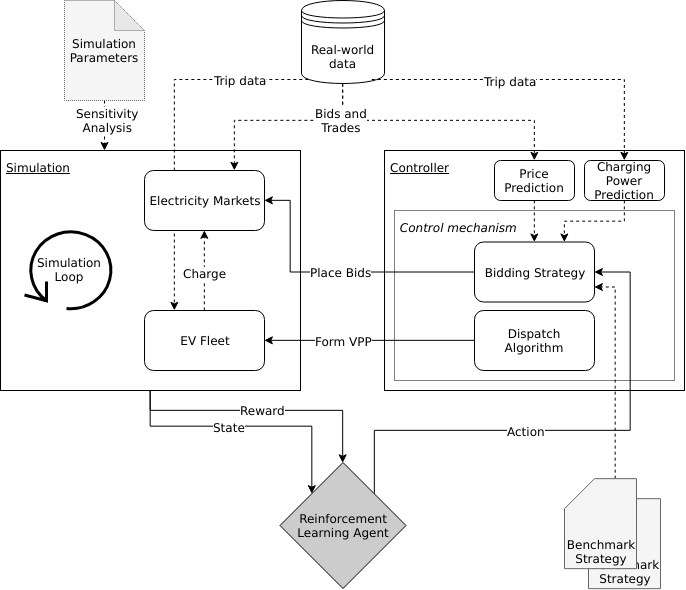
\includegraphics[width=1\linewidth]{./fig/simulation_platform.png}
\caption[FleetSim Architecture]{Architecture of FleetSim \label{fig-fleetsim}}
\end{figure}

\subsection{Modular Expandability}
\label{sec:org21b5f0e}
\begin{itemize}
\item Plug-in different Market designs
\item Use different real-world data
\item Change Fleet parameters
\item Develop new strategy
\item
\end{itemize}

\clearpage
\section{Results}
\label{sec:orgd5b69ea}
\subsection{Simulation Settings}
\label{sec:orga7ac8fb}
\begin{itemize}
\item Results heavily dependent on industry charging price, since on average the
balancing prices are 50\% cheaper, and intraday 30\% cheaper.
\item BMWi. (n.d.). Prices of electricity for the industry in Germany from 2008 to
2017 (in euro cents per kilowatt hour). In Statista - The Statistics Portal.
Retrieved March 18, 2019, from
\url{https://www.statista.com/statistics/595803/electricity-industry-price-germany/}.
\end{itemize}
\subsection{FleetRL}
\label{sec:orgd10220f}
\begin{itemize}
\item long-delayed rewards make RL hard (!?)
\end{itemize}
\subsection{Sensitivity Analysis}
\label{sec:orgc9aecc9}
\begin{itemize}
\item Prediction Accuracy
\end{itemize}

\begin{itemize}
\item Charging infrastructure
\end{itemize}
\section{Conclusion}
\label{sec:orgad49553}
\subsection{Contribution}
\label{sec:org4f90cb4}
\begin{itemize}
\item Compare to most simular studies:
\end{itemize}
\cite{kahlen18_elect_vehic_virtual_power_plant_dilem,vandael15_reinf_learn_heuris_ev_fleet} etc..
\begin{itemize}
\item Business model for EV fleet owners with better results than previous studies
\item Environmental impact by providing balancing power
\item Decision Support System for controlled EV charging from multiple markets
\item RL Algorithm that is designed to work in previously unknown environments and
thus suited to deploy in real life settings of all kinds of EV fleets in all
kinds of cities. E.g. scooters also?
\item Event-based Simulation Platform to evaluate bidding strategies and RL agents,
facilitate research
\end{itemize}

\subsection{Limitations}
\label{sec:org3c47591}
\begin{itemize}
\item Model:
\begin{itemize}
\item Bidding Mechanism: one week ahead, always accepted
\item Policy \& Regulation: EVs not allowed to provide balancing power, minimum
bidding quantities 1MW.
\item Markets: Fleet is a price-taker, what about larger fleets? Simulate market influence
\end{itemize}
\item RL: See \cite{vazquez-canteli19_reinf_learn_deman_respon} conclusion for
limitations.
\end{itemize}
\subsection{Future Research}
\label{sec:org9053b83}
\begin{itemize}
\item Model: Current market design, i.e. daily w/ 4h slots. German "Mischpreisverfahren"
\item RL: Long-delayed rewards, different reward structure, memory based
\end{itemize}

\clearpage
\bibliography{bibliography/references}
\bibliographystyle{apacite}
\end{document}
